\documentclass{book}

\usepackage{etoolbox}

\makeatletter
\def\subtitle#1{\gdef\@subtitle{#1}}
\patchcmd\maketitle
  {{\LARGE \@title \par}}
  {{\LARGE \@title \par}%
   \vskip 1.5em
   {\Large \@subtitle \par}}
\makeatother

\usepackage[utf8x]{inputenc}
\usepackage{amsmath,mathtools}
\usepackage{amsfonts}
\usepackage{amssymb}
\usepackage{graphicx}
\usepackage{appendix}
\usepackage{bm}
\usepackage{multicol}
\usepackage{geometry}
\usepackage{colortbl}
\usepackage{changepage}
\usepackage{color}
\usepackage{mathrsfs}
\usepackage{bigints}
\usepackage{pdflscape}
\usepackage{adjustbox}
\usepackage{tocloft}
\usepackage{lscape}
\usepackage[dvipsnames]{xcolor}
\usepackage[colorlinks=true,
            linkcolor=blue,
            urlcolor=blue,
            citecolor=blue]{hyperref}

\sloppy
\usepackage{tikz, lipsum}% http://ctan.org/pkg/{pgf,lipsum}
\newcommand*{\chapnumfont}{\normalfont\sffamily\huge\bfseries}
\newcommand*{\printchapternum}{
  
\begin{tikzpicture}
    \draw[fill,color=gray75] (0,0) rectangle (2cm,2cm);
    \draw[color=white] (1cm,1cm) node { \chapnumfont\thechapter };
  \end{tikzpicture}
}
\newcommand*{\chaptitlefont}{\normalfont\sffamily\Huge\bfseries}
\newcommand*{\printchaptertitle}[1]{\flushright\chaptitlefont#1}

\makeatletter
% \@makechapterhead prints regular chapter heading.
% Taken directly from report.cls and modified.
\def\@makechapterhead#1{%
  \vspace*{50\p@}%
  {\parindent \z@ \raggedleft
    \ifnum \c@secnumdepth >\m@ne
        \printchapternum
        \par\nobreak
        \vskip 20\p@
    \fi
    \interlinepenalty\@M
    \printchaptertitle{#1}\par\nobreak
    \vskip 40\p@
  }}
% \@makeschapterhead prints starred chapter heading.
% Taken directly from report.cls and modified.
\def\@makeschapterhead#1{%
  \vspace*{50\p@}%
  {\parindent \z@ \raggedleft
    \interlinepenalty\@M
    \printchaptertitle{#1}\par\nobreak
    \vskip 40\p@
  }}
\makeatother


\renewcommand\contentsname{}

\definecolor{gray75}{gray}{0.75}

\title{\Huge \bfseries\sffamily Diffusing ideas}
\subtitle{\Large \bfseries\sffamily \color{gray75} Adventures with noise and building mathematical toys}
\author{\bfseries\sffamily Robert J. Hardwick}
\date{\today}
\begin{document}
\maketitle
\frontmatter

\chapter*{Introduction}

\emph{Diffusing ideas} records a journey of research exploration and software development. It expresses a collection of interrelated ideas around the statistical inference and automated control of stochastic phenomena and, in order to manifest these ideas into reality, the project has involved designing and building a lot of new open-source scientific software. The motivation behind developing these computational elements is to form a foundation from which one can build a variety of new applications, and to make researching new phenomena much more efficient. Testing and experimentation has also led to some fun digressions into a range of interesting mathematical toy models which are motivated by the real world, which we hope that the reader will enjoy exploring them as well!

Any software that is described in this book will always be shared under a \href{https://opensource.org/licenses/MIT}{MIT license} in the following public git repository: \href{https://github.com/umbralcalc}{https://github.com/umbralcalc}. In all cases, note that the code should still be considered as very much `in development' and so it is advised that it is not deployed in a production pipeline without careful scrutiny at the user's own risk. 

No quest would be complete without a map, so in this introductory section, we will now outline some of the key milestones of the book and their motivations within the context of the overall research project. Our core aims can be divided into answering 4 interdependent research questions in the following order:

\begin{enumerate} 
\item{How do we simulate a general set of stochastic phenomena?}
\item{How do we then learn/identify 1. from real-world data?}
\item{How do we simulate a general set of automated control policies to interact with 1.?}
\item{How do we then optimise 3. to achieve a specified control objective?} 
\end{enumerate}




\chapter*{Table of contents}
\vspace*{-3cm}
{\sffamily \tableofcontents}
\mainmatter



\chapter{\sffamily Building the `stochadex'}

\vspace*{1cm}
{\bfseries\sffamily Concept.} The idea here is 

\vspace*{1cm}
\section{\sffamily Core mathematical formalism}

Ideally, the stochadex sampler should be designed to try and maintain a balance between performance and flexibility of utilisation (it's meant to be a general stochastic modelling tool after all!). But before we dive into the software, we need to define the mathematical approach we're going to take. It seems reasonable to start with writing down the following formula which describes iterating some arbitrary process forward in time (by one finite step) and adding a new row each to some matrices $S' \rightarrow S$ and $X' \rightarrow X$
%%
\begin{align}
& X^i_{t+\delta t} = F^i_{t+\delta t}(X',t) + S^i_{t+\delta t}(X',S',t)\,,
\end{align}
%%
where to explain things in a bit more detail, let's define

\begin{itemize}
\item[]{$\delta t$ as the size of the next timestep}
\item[]{$i$ as an index for the dimensions of the 'state' space}
\item[]{$t$ as the current time which may either correspond to the index for some arbitrary stepping process (where $\delta t = 1$), or the explicit time variable for a discrete-time process or some discrete approximation to a continuous-time process}
\item[]{$X$ as the next version of $X'$ after one timestep (and hence one new row has been added)}
\item[]{$S$ as the next version of $S'$ (similarly to $X$ and $X'$)}
\item[]{$F^i_{t+\delta t}(X', t)$ as the latest element of some matrix which very generally can depend on $X'$, $t$ and $\delta t$}
\item[]{$S^i_{t+\delta t}(X', S', t)$ as the recorded values of a stochastic process defined over the dimensions of the state space indexed by $i$ which may either vary with continuous sample paths in time or not, and which very generally can depend on $X'$, $S'$, $t$ and $\delta t$.}
\end{itemize}

So the idea here is to iterate the matrices $X$ and $S$ forward in time by a row, and use their previous versions ($X'$ and $S'$) as entire matrix inputs into functions which populate the elements of their latest rows. Note that I've avoided using the time variable $t$ and its step size $\delta t$ (reducing the formalism to that of an arbitrary stepping process) to try and make the diagram above more clear, but, more generally, these values may be present in the calculations of new matrix rows.

Why go to all this trouble of storing matrix inputs for previous values of the same process? For a large class of stochastic processes this memory of past values is essential to consistently construct the sample paths moving forward. This is true in particular for \emph{non-Markovian} phenomena (see, e.g., \href{https://en.wikipedia.org/wiki/Markov_chain}{Markov chains} to get a sense of their antithesis), where the latest values don't just depend on the immediately previous ones but can depend on values which occured much earlier in the process.

\section{\sffamily Flavours of noise with continuous sample paths}

For \emph{Wiener process noise}, adopting the \href{https://en.wikipedia.org/wiki/It\%C3\%B4_calculus}{Itô interpretation} in this section, we can define $W^i_{t}$ is a sample from a Wiener process for each of the state dimensions indexed by $i$ and our formalism becomes
%%
\begin{align}
& X^i_{t+\delta t} = F^i_{t+\delta t}(X', t) + \textcolor{red}{W^i_{t+\delta t}-W^i_{t}}\,.
\end{align}
%%

Other interpretations of the noise are less immediately compatible with our formalism as it is currently written, e.g., \href{https://en.wikipedia.org/wiki/Stratonovich_integral}{Stratonovich} or others within the $\alpha$-family, but it seems less necessary to complicate the details of this section further, so we'll just cover these extensions at the software implementation level. Note also that we may also allow for correlations between the noises in different dimensions. 

For \emph{Geometric Brownian motion noise}, we simply have
%%
\begin{align}
& X^i_{t+\delta t} = F^i_{t+\delta t}(X', t) + \textcolor{red}{X^i_{t}(W^i_{t+\delta t}-W^i_{t})}\,.
\end{align}
%%

And say, e.g., \emph{fractional Brownian motion noise}, where $B^i_{t}({H_i})$ is a sample from a fractional Brownian motion process with Hurst exponent $H_i$ for each of the state dimensions indexed by $i$, we simply substitute again
%%
\begin{align}
& X^i_{t+\delta t} = F^i_{t+\delta t}(X', t) + \textcolor{red}{B^i_{t+\delta t}({H_i})-B^i_{t}({H_i})}\,.
\end{align}
%%

\emph{Generalised continuous noises} would take the form
%%
\begin{align}
& X^i_{t+\delta t} = F^i_{t+\delta t}(X', t) + \textcolor{red}{g^i_{t+\delta t}(X', W^i_{t+\delta t}-W^i_t, \dots)}\,,
\end{align}
%%
where $g^i_{t+\delta t}(X', W^i_{t+\delta t}-W^i_t, \dots)$ is some continuous function of its arguments which can be expanded out with \href{https://en.wikipedia.org/wiki/It\%C3\%B4\%27s_lemma}{Itôs Lemma}.


\section{\sffamily Flavours of noise with discontinuous sample paths}

\emph{Jump process noises} generally could take the form
%%
\begin{align}
& X^i_{t+\delta t} = F^i_{t+\delta t}(X', t) + \textcolor{red}{J^i_{t+\delta t}(X', \dots )}\,,
\end{align}
%%
where $J^i_{t+\delta t}(X', \dots )$ are samples from some arbitrary jump process (e.g., compound Poisson) which could generally depend on a variety of inputs, including $X'$. 

\emph{Poisson process noises} would generally take the form
%%
\begin{align}
& X^i_{t+\delta t} = F^i_{t+\delta t}(X', t) + \textcolor{red}{N^i_{t+\delta t}({\lambda_i})-N^i_{t}({\lambda_i})}\,,
\end{align}
%%
where $N^i_{t}({\lambda_i})$ is a sample from a Poisson process with rate $\lambda_i$ for each of the state dimensions indexed by $i$. Note that we may also allow for correlations between the noises in different dimensions.

\emph{Time-inhomogeneous Poisson process noises} would generally take the form
%%
\begin{align}
& X^i_{t+\delta t} = F^i_{t+\delta t}(X', t) + \textcolor{red}{N^i_{t+\delta t}({\lambda^i_{t+\delta t}})-N^i_{t}({\lambda^i_t})}\,,
\end{align}
%%
where $\lambda^i_{t}$ is a deterministically-varying rate for each of the state dimensions indexed by $i$.

\emph{Cox (doubly-stochastic) process noises} would generally take the form
%%
\begin{align}
& X^i_{t+\delta t} = F^i_{t+\delta t}(X', t) + \textcolor{red}{N^i_{t+\delta t}({\Lambda^i_{t+\delta t}})-N^i_{t}({\Lambda^i_{t}})}\,,
\end{align}
%%
where the rate $\Lambda^i_{t}$ is now a sample from some continuous-time stochastic process (in the positive-only domain) for each of the state dimensions indexed by $i$.

\emph{Self-exciting process noises} would generally take the form
%%
\begin{align}
& X^i_{t+\delta t} = F^i_{t+\delta t}(X', t) + \textcolor{red}{N^i_{t+\delta t}[{\cal I}^i_{t+\delta t}(N', \dots)]-N^i_{t}[{\cal I}^i_{t}(N'', \dots)]}\,,
\end{align}
%%
where the stochastic rate ${\cal I}^i_{t}(N', \dots)$ now depends on the history of $N'$ explicitly (amongst other potential inputs - see, e.g., \href{https://en.wikipedia.org/wiki/Hawkes_process}{Hawkes processes}) for each of the state dimensions indexed by $i$.

\emph{Generalised probabilistic discrete state transitions} would take the form
%%
\begin{align}
& X^i_{t+\delta t} = \slash{F^i_{t+\delta t}(X', t)} + \textcolor{red}{T^i_{t+\delta t}(X')}\,,
\end{align}
%%
where $T^i_{t+\delta t}(X')$ is a generator of the next state to occupy. This generator uses the current state transition probabilities (which are generally conditional on $X'$) at each new step.

\section{\sffamily Summary of desirable features}

\begin{itemize}
\item{using the learnings from the previous sections looking at specific example processes}
\item{above formalism is so general that it can do anything - so while it shall serve as a useful guide and reference point, it would be good here to go through more of the specific desirable components we want to have access to in the software itself}
\item{it might not always be convenient to have the windowed histories stored as S but some other varying quantity which can be used to construct S? take fractional brownian motion as an example of this! hence, need to provide more possible input histories into S}
\item{want the timestep to have either exponentially-sampled lengths or fixed lengths in time}
\item{formalism already isn't explicit about the choice of deterministic integrator in time}
\item{but also want to be able to choose the stochastic integrator in continuous processes (Itô or Stratonovich?)}
\item{enable correlated noise terms at the sample generator level}
\item{configurable setup of simulations with just yamls + a single .go file defining the terms}
\end{itemize}


Test cite~\cite{Dimastrogiovanni:2018xnn}

\section{\sffamily Software design choices}

\chapter{\sffamily Building a Rugby simulator game}

\vspace*{1cm}
{\bfseries\sffamily Concept.} The idea here is 

\vspace*{1cm}
\section{\sffamily Introduction}

Since the basic game engine will run using the \href{https://github.com/umbralcalc/stochadex}{stochadex} sampler, the novelties in this project are all in the design of the rugby match model itself. And, in this instance, I'm not especially keen on spending a lot of time doing detailed data analysis to come up with the most realistic values for the parameters that are dreamed up here. Even though this would also be interesting.

One could do this data analysis, for instance, by scraping player-level performance data from one of the excellent websites that collect live commentary data such as \href{https://www.rugbypass.com/}{rugbypass.com} or \href{https://www.espn.co.uk/rugby/}{espn.co.uk/rugby}.

This game is primarily a way of testing out the interface of the stochadex for other users to build projects with. This should help to both iron out some of the kinks in the design, as well as prioritise adding some more convenience methods for event-based modelling into its code base.

\section{\sffamily Designing the event simulation engine}

We need to begin by specifying an appropriate event space to live in when simulating a rugby match. It is important at this level that events are defined in quite broadly applicable terms, as it will define the state space available to our stochastic sampler and hence the simulated game will never be allowed to exist outside of it. So, in order to capture the fully detailed range of events that are possible in a real-world match, we will need to be a little imaginative in how we define certain gameplay elements when we move through the space.

The diagrams below sum up what should hopefully work as a decent initial approximation while providing a little context with specific examples of play action.

\begin{figure}[h]
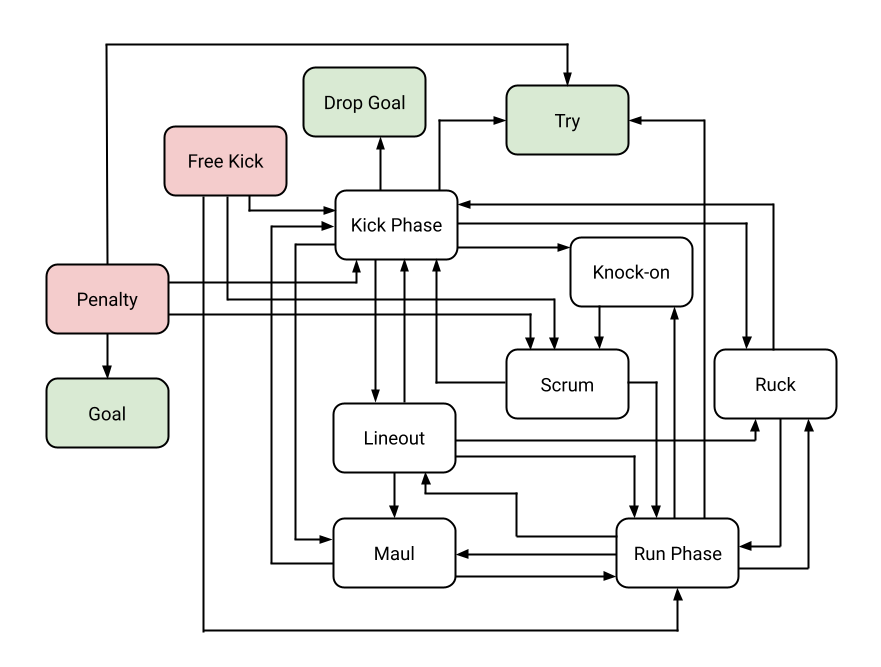
\includegraphics[width=8cm]{images/trywizard-event-graph.png}
\caption{Simplified event graph of a rugby union match.}
\label{fig:event-graph}
\end{figure}

\begin{figure}[h]
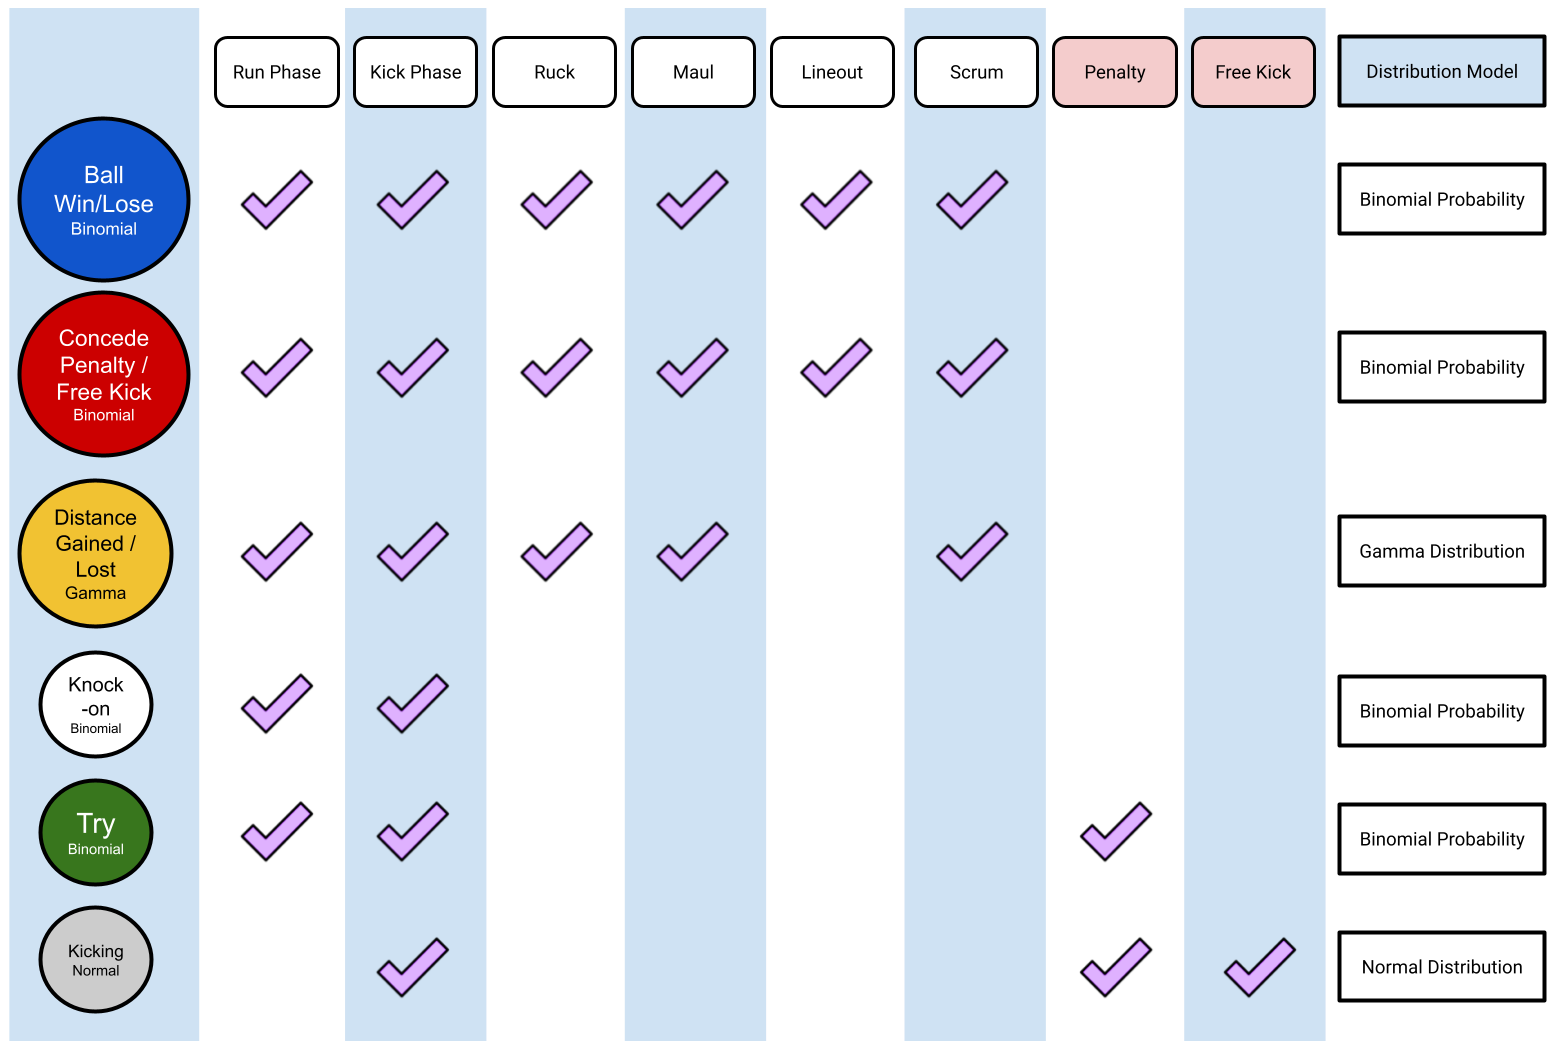
\includegraphics[width=10cm]{images/trywizard-model-ideas-sketch.png}
\caption{Optional model ideas.}
\label{fig:model-ideas}
\end{figure}

\section{\sffamily Linking to player attributes}

\section{\sffamily Deciding on gameplay actions}

\section{\sffamily Writing the game itself}

%\appendix
%\chapter{First and only appendix}
\backmatter
\chapter*{Bibliography}
\bibliographystyle{JHEP}
\bibliography{book}
\end{document}